%----------------------------------------------------------------------------------------
%   Theoretical Framework (Probleemanalyse)
%
%----------------------------------------------------------------------------------------
\chapter{Theoretical Framework}

%----------------------------------------------------------------------------------------
%   Introduction
%----------------------------------------------------------------------------------------
\section{Introduction}
To determine the difference in workload, and in-depth review of Peppr's current workflow is needed. Below is a deep-dive into the process currently used, split into a graphics and software section. A detailed outline of the 3d process will be described in the graphics section, while a peek into the software development process will be described in the software section. The split into these components will make it easier to determine possible sections of improvement later on.
Apart from the current workflow, a basic understanding of possible new technologies needs to be looked at, as well as the current market position with regards to the technologies hype-cycle and acceptance.

%----------------------------------------------------------------------------------------
%   Workflow
%----------------------------------------------------------------------------------------
\clearpage
\section{Workflows}
Peppr has done these projects and states that the usual way of building consist of two main parts. One being the images, the other, the software. In the outline below follows a brief description of how the process is currently done. 

For this thesis, we will use an example to show the differences. Please note that this process is the way Peppr handles projects like this, and, while they did try to optimise it, they in no mean imply this is the perfect way to tackle such a project. 

\say{
A chair manufacturer wants a product configurator for one of their most popular chairs. It has 25 different colour options and has 4 different subframes. Two of the subframes are steel and can be either black or plain. The other two have wooden elements and have four wood colour options.
}


%----------------------------------------------------------------------------------------
%   Graphics
%----------------------------------------------------------------------------------------
\subsection{Graphics}

%----------------------------------------------------------------------------------------
%   Image Planning
%----------------------------------------------------------------------------------------
\subsubsection{Image Planning}
Product configurators may have to deal with an exponentially growing set of options. Peppr always checks if these image sets can be split into separate components. This may make the set smaller and easier to maintain. Below is a summary of the option set, split per item so we can start calculating how many images will be necessary.
\begin{itemize}
	\item 25 colours - \textbf{(\( \alpha \))}
	\item 2 steel frames - \textbf{(\( \beta \))}
	\item 2 frame colours - \textbf{(\( \gamma \))}
	\item 2 wood frames - \textbf{(\( \delta \))}
	\item 4 wood colours - \textbf{(\( \epsilon \))}
\end{itemize}

In this case, any seat has a pick of several frame options, and several colours. But steel frames have two colours and wood frames have four colours. To calculate the full amount of options ($x$), we can use the following formula:
 
\[ f(x) = (\alpha \cdot \beta \cdot \gamma) + (\alpha \cdot \delta \cdot \epsilon)\]
\[ f(x) = (25 \cdot 2 \cdot 2) + (25 \cdot 2 \cdot 4)\]
\[ f(x) = 300\]

Going with just 1 colour more adds 12 extra renders. While this does not seem like much, these renders are built from several different files. This means an artist has to open 12 different files, and do the edit 12 times.
In some cases, you might be able to get around it using layers. In this case, splitting up the chair into a seat and frame layer will get us the following formula:

\[ f(x) = (\alpha) + (\cdot \beta \cdot \gamma) + (\cdot \delta \cdot \epsilon)\]
\[ f(x) = (25) + (2 \cdot 2) + (2 \cdot 4)\]
\[ f(x) = 37\]

This decreases the amount of renders. Unfortunately, while this works here, in some cases this is not possible. Sometimes, one of the objects is both in front and behind other objects. This makes it difficult to 'mask' and makes proper reflections tricky. Also, creating new layers does add complexity and constraints. Adding new options and layers might prove difficult when they overlap with existing layers.
\newline
Apart from difficulties in the 3d process, these layers need to be added to the software as well. Either by creating an API that serves the layers as one image (\cite{bugaboo} ), or by stacking the images client-side. The user will notice this option though, as it slows things down. This is fixed with the adoption of HTTP 2.0. This pipelines the http-requests, reducing latency (\cite{latency}).

%----------------------------------------------------------------------------------------
%   Modeling
%----------------------------------------------------------------------------------------
\subsubsection{Modeling}

\begin{wrapfigure}[12]{r}{10cm}
\vspace{-1cm}
\centering
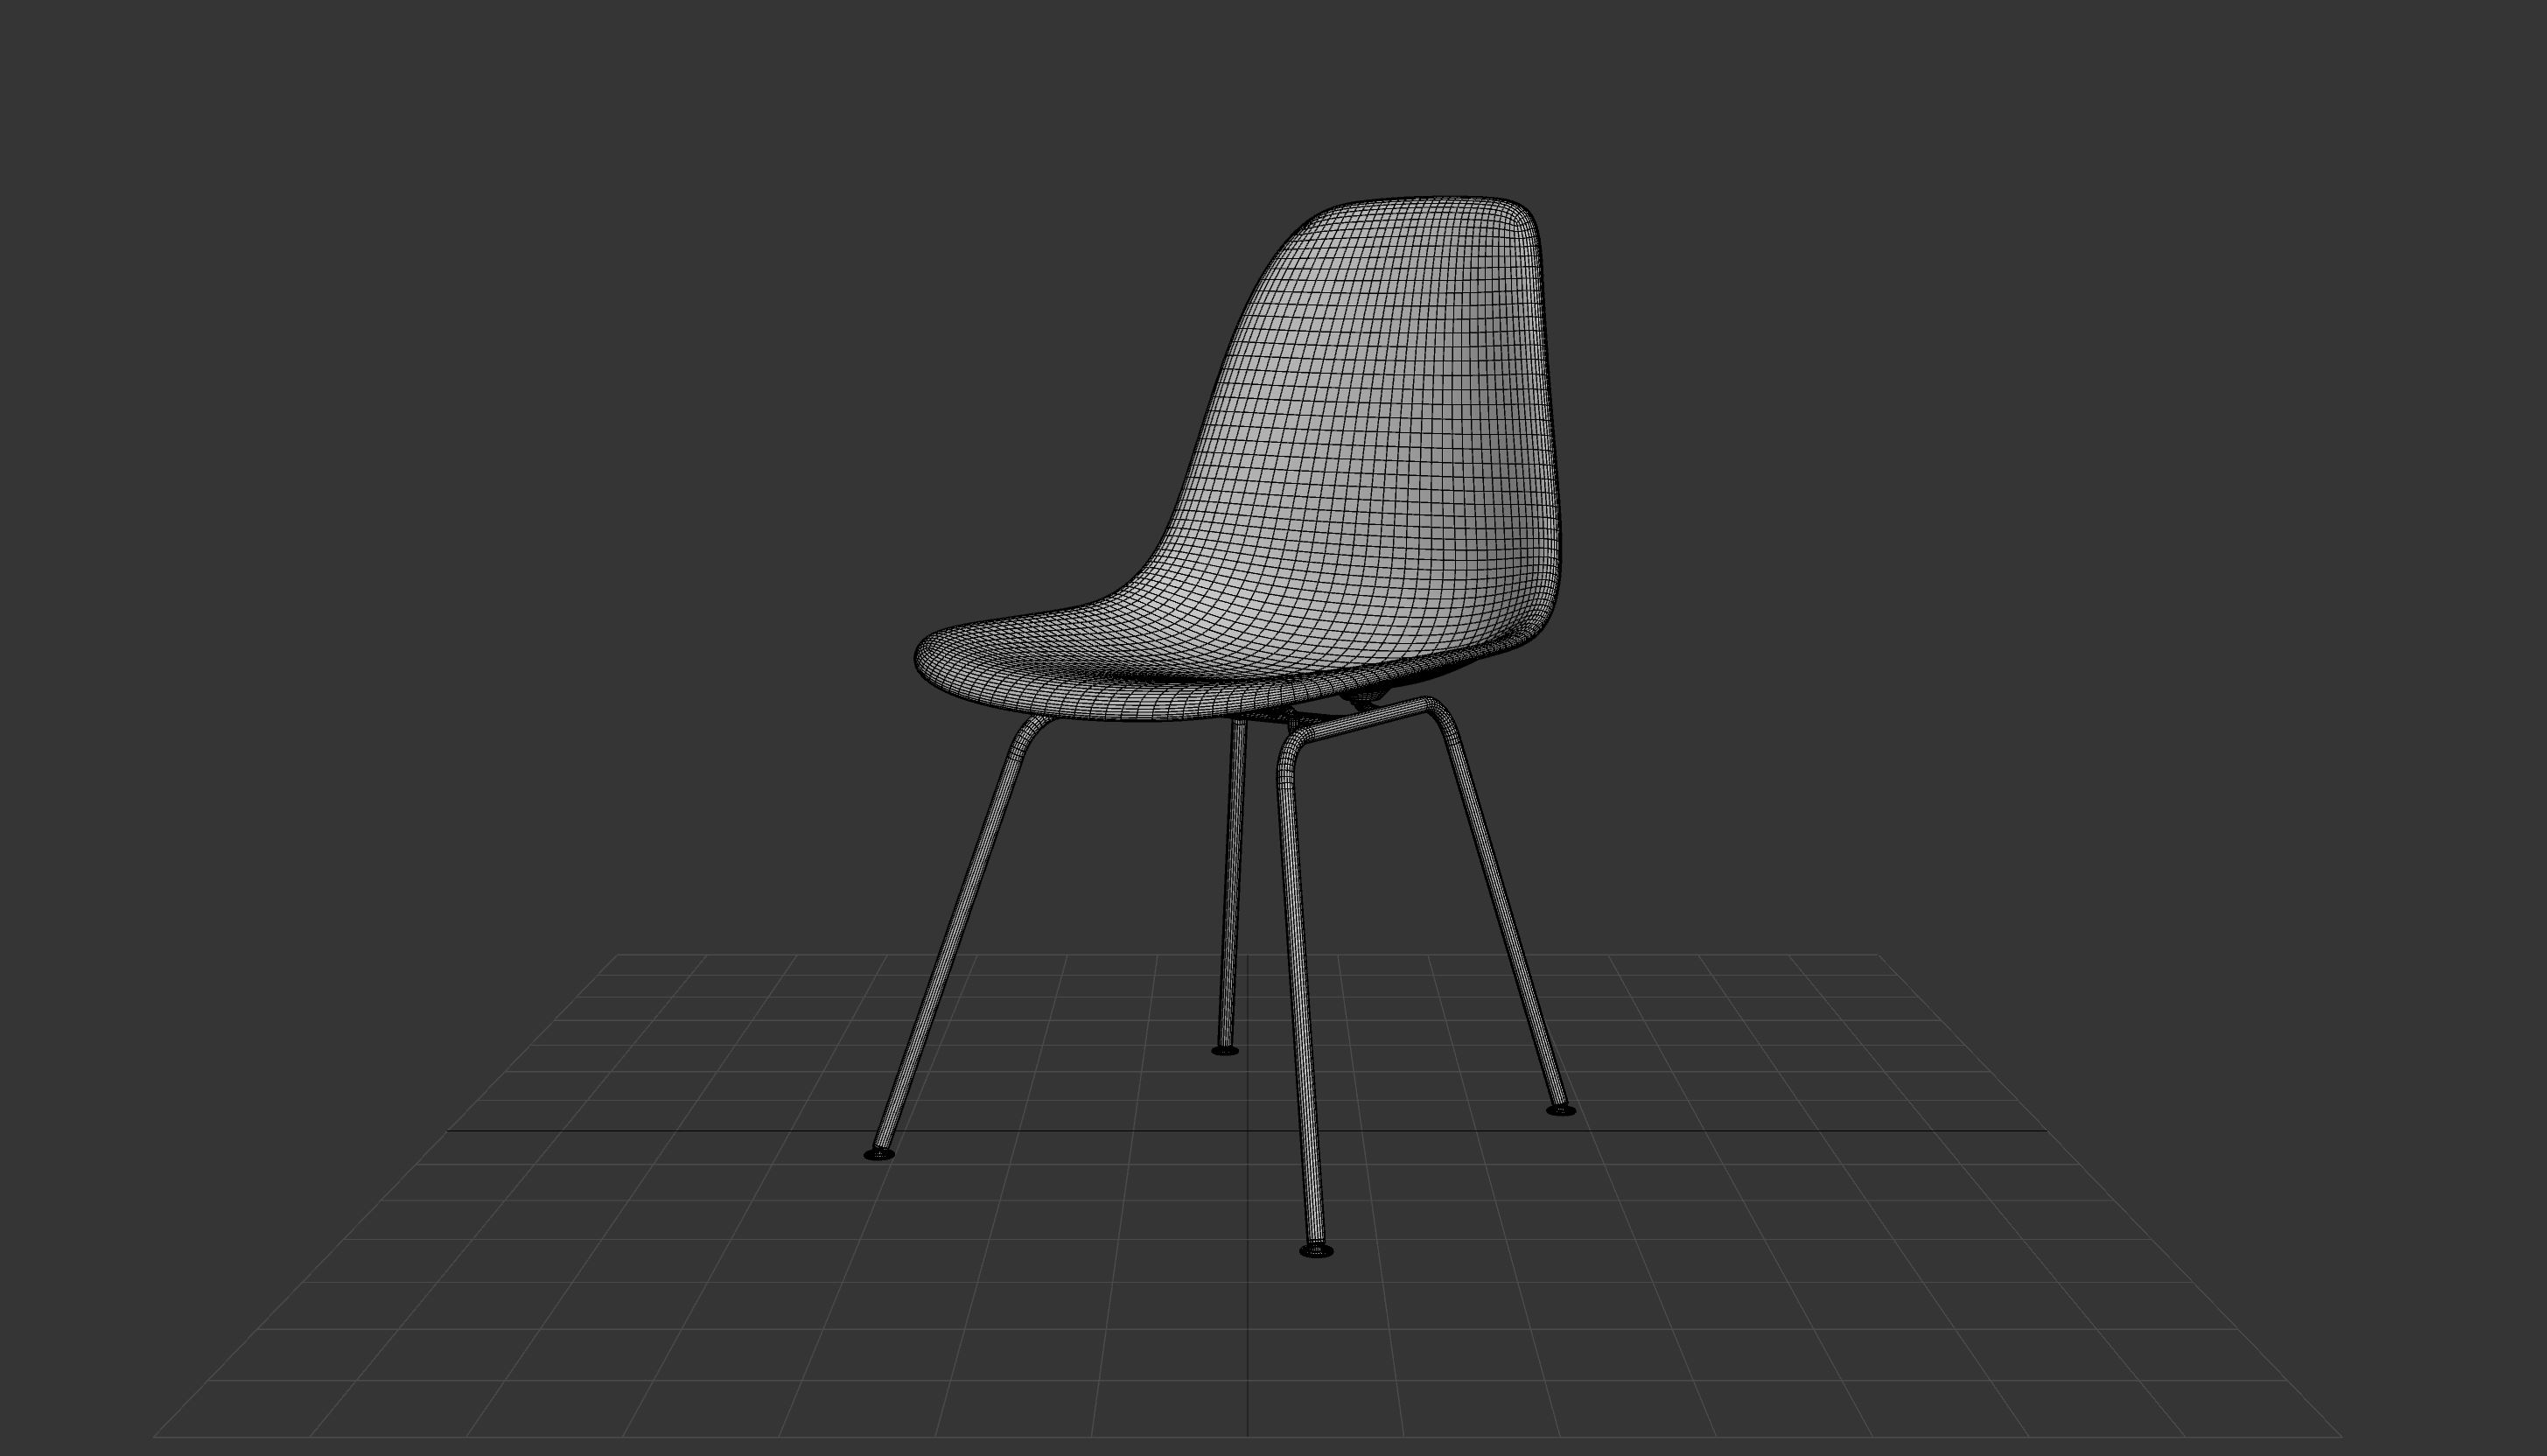
\includegraphics[width=9cm]{images/modeling}
\caption{Lighting Setup}
\label{figure:modeling}
\end{wrapfigure}


Step two in the process is modeling, whereby an artist makes a virtual model. Mostly used at Peppr is a form of modeling called Polygonal modeling. This means the model will eventually be represented by an array of 3 dimensional points (or vertices). All vertices are connected by lines and those lines make up the surface of the model. There are multiple ways of creating these models, an artist may choose to 'draw' those polygons from scratch, but may also use 3d scanning services or even simulations to build the 3d models.
As seen in \ref{figure:modeling}, every single square in that model is one of those polygons.

%----------------------------------------------------------------------------------------
%   Lighting / Shading
%----------------------------------------------------------------------------------------
\clearpage
\begin{figure}
\centering
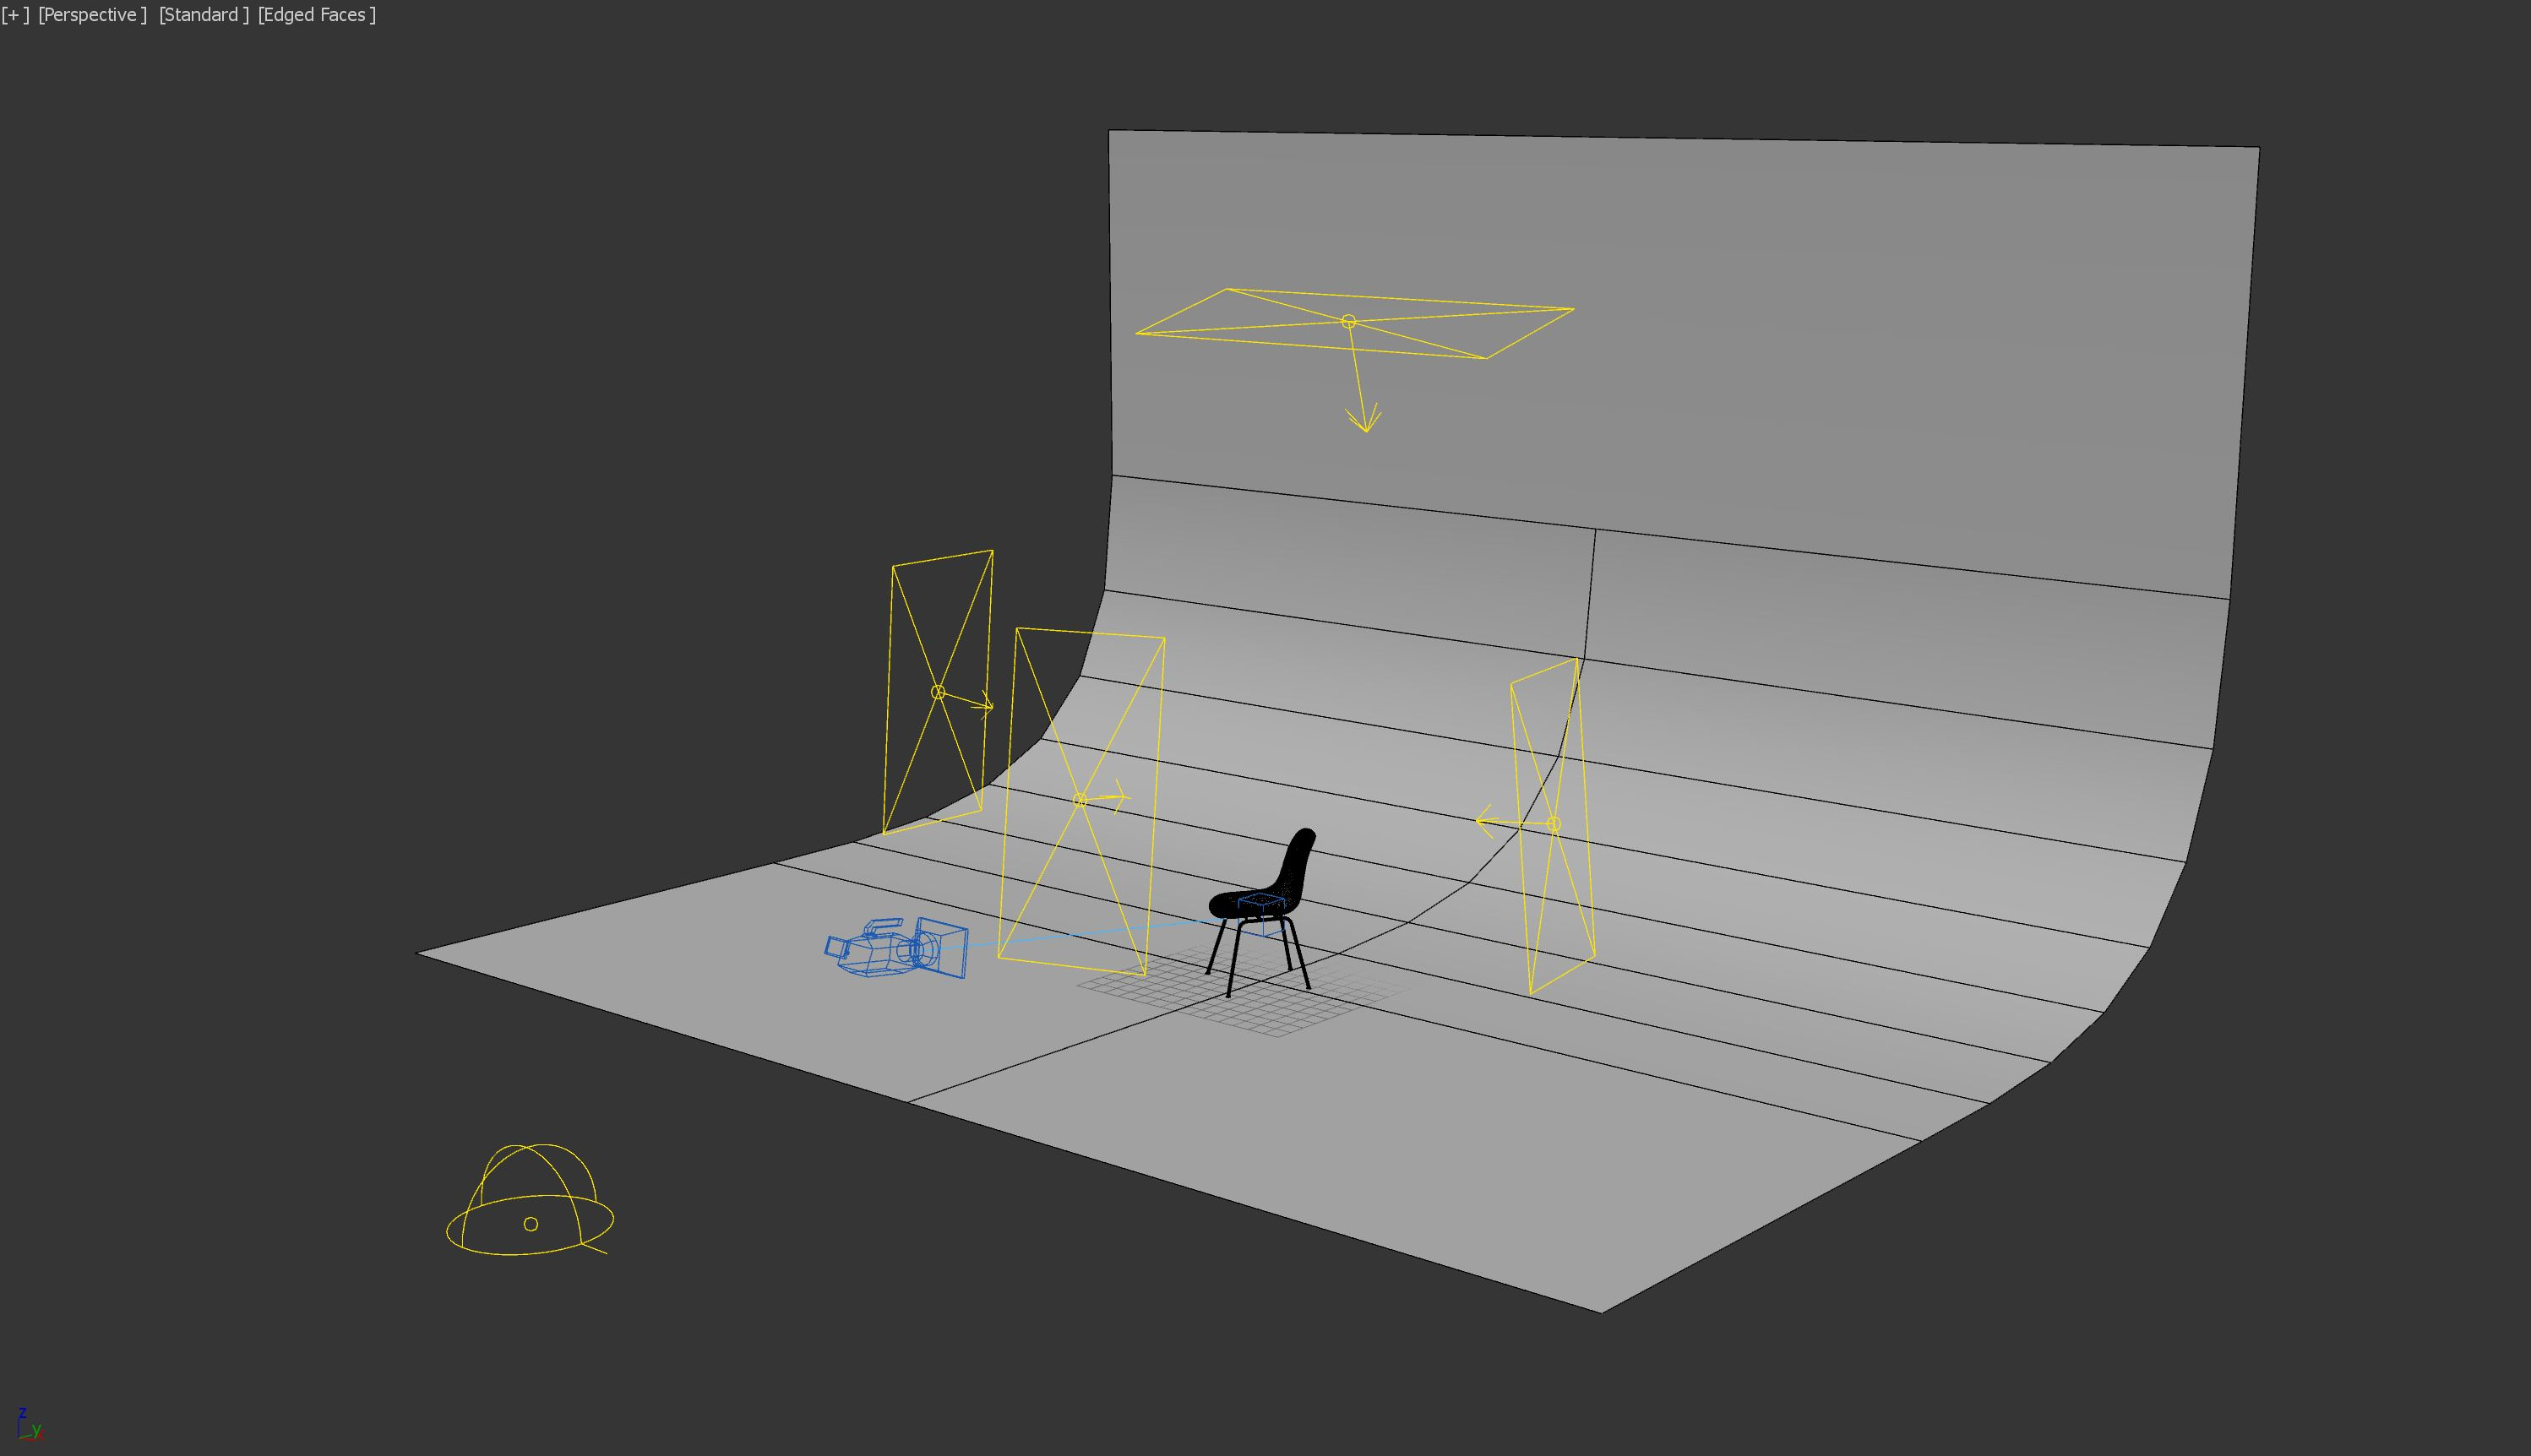
\includegraphics[width=15cm]{images/lighting}
\caption{Lighting Setup}
\label{figure:lighting}
\end{figure}


\subsubsection{Lighting}

\begin{wrapfigure}[12]{r}{10cm}
\vspace{-1cm}
\centering
\includegraphics[width=9cm]{images/lighting_rendered}
\caption{Rendered Lighting Setup}
\label{figure:lighting_rendered}
\end{wrapfigure}

Once in the lighting department, the model is placed into a virtual environment. Most of the time this environment will simulate a photography studio. As seen in figure \ref{figure:lighting}, there are 5 lights in the current setup. One is a dome light that simulates the environment using a so-called 'High Dynamic Range' (HDR) range image. Current .JPG images are 24 bit. As an image is separated into a red, green and blue channel, every colour has 8 bits of information available. This means a jpg image is able to show 256 ($2^8$) shades per colour, so a normal JPG image has $16.777.216$ possible colours in total. \newline
The HDR images are mostly encoded in a 32 bits per pixel option. In laymen terms, this means that an HDR image has more colours per pixel ($4.294.967.296$), than a JPG image has in total. In practice, this means that the extremely bright parts of the image can be used to extract lighting information. The HDR image is mapped onto a spherical dome, which results in the ability to mimic environments without the need for additional lighting. In this case, Peppr used an actual studio environment for that part.
 The other four images are used to light the model to perfection. One on the back to light the background, one in front to have highlights and two diffuse boxes on the side to get the model to stand out from the background.

%----------------------------------------------------------------------------------------
%   Lighting / Shading
%----------------------------------------------------------------------------------------

\subsubsection{Shading}

\begin{wrapfigure}[16]{r}{10cm}
\vspace{-1cm}
\centering
\includegraphics[width=9cm]{images/rendering}
\caption{Rendered image with shaders}
\label{figure:lighting_rendered}
\end{wrapfigure}

Once properly lit, an artist will start shading the model. This is the process of adding life-like materials to the object and making it come to life. This process can be tricky as there are loads of variables involved. Diffuse colour, reflectivity, refractivity but also slight bumps and anisotropy have to be taken into consideration.


%----------------------------------------------------------------------------------------
%   Rendering
%----------------------------------------------------------------------------------------
\subsubsection{Render}
This is where things get together and the calculation from 3d model to actual image start. There are two sides to this, the technical settings of the render-engine used and the structure of the file / timeline.
\newline
\textit{Render-engine}
\newline
Peppr opts to use third party render-engines for their projects, mostly due to the speed and quality optimizations. While more configurable, they are also more difficult to use. Many times, there is an equilibrium between quality and render-times. The high render-times have to do with the difficult nature of lights, reflections, refractions and the anti-aliasing of the image. Light for instance, obeys the 'inverse square law' (\cite{inverseLightLaw}), this means the intensity of light decays the further it gets from the point-of-origin. With one light this is quite easy, but imagine having 3 or 10 lights interacting at different intensities from different point-of-views. On top of that, light bounces around. The render-engine will calculate the point of impact, check the properties of the materials it hits and radiate the light back from the surface. The directionality of these light reflections is where things get tricky. The more straightforward the reflections, the easier. A mirror will reflect the light at the same angle of incidence, but when the material is rough, the rays get scattered. For this, the render-engine will sent out multiple rays (for example 50), up to a predefined amount of times. In practice, this may mean that when one ray bounces on a rough surface, it spawns 50 new rays. If all of those rays bounce off of a rough surface again, the rays will amount to 50 x 50. With every bounce, this will increase exponentially.

Refractions makes these things even more tricky because of the Index of Refraction. This specifies change of angle in the lights ray when it goes from one material to another (\cite{refractiveIndex}). Water (at 20c) for instance, has an IOR of 1.333 (\cite{waterIOR}). This means that next to the light rays bouncing, they can also change direction.

The third and last part that makes rendering images a painstakingly long task is anti-aliasing. Anti-aliasing is a way of making the images 'smooth'. It has to do with the square nature of pixels. A diagonal line will not look smooth if it is just one line of pixels. Instead, the pixels directly surrounding it get a semi-translucent fill, which makes the line look smooth. The blending of colours (while not overdoing it) is the anti-aliasing part.

Peppr uses these intricate render-engines to fine-tune the render-settings. For studio setups, where direct lights are the most important light sources, Peppr might choose to use a set of settings where the secondary bounces of light are of lesser quality than for instance an interior, where most light comes from the light bouncing on the floor (mostly indirect).
\newline
\newline
\textit{Automation}
\newline
Sometimes it is easier to render out the whole sequence with every configuration. Other times, it is easier to render just one point-of-view at a time. In the case of the shirt configurator, every shirt had loads of different collars, sleeves, buttons, but also colours. There are numerous ways of splitting this up, automating the process as much as possible. Most 3d applications allow for animations. By changing one aspect of the model for every rendered frame and rending it out as an image sequence, the rendering process can be automated (a bit). The problem with this is that it will always be a choice of lesser evils. While rendering the sequence, it is important to have the most changes possible rendered at once. In the shirt configurator case, this meant splitting it up so that there is a file for every colour. In that way, the file structure is somewhat logical (a file for every colour) and changing one aspect is relatively easy (changing it once, and applying it to the 25 different colours). Unfortunately, this is by no means ideal. Some changes have to be done 25 times (one for every colour).


%----------------------------------------------------------------------------------------
%   Post Production
%----------------------------------------------------------------------------------------
\subsubsection{Post Production}
Every 3d model needs a bit of post production to make it look better. If the model has layers rendered as masks (an option to overcome overlapping images). This is the step where they would split them into the different layers. In case of the shirt configurator, this has partly been automated. Using the same animation principles highlighted in the 'Render' section, Peppr made sure they would have one file per colour so they could easily copy changes from one set of colours to another.
\newline
%----------------------------------------------------------------------------------------
%   Compression
%----------------------------------------------------------------------------------------
\subsubsection{Compression}
Using images on the web, especially on bigger resolution displays, small file sizes are important. Current mobile data speeds and capped contracts are difficult. So laying a 50mb burden upon the user when opening a site is not a good idea. According to the W3C guidelines, the file size should not exceed 20 kilobytes (\cite{pageFileSizeLimit}). This is were compression comes in. Every images gets compressed for a fast download, while remaining a good quality.

%----------------------------------------------------------------------------------------
%   Aims
%----------------------------------------------------------------------------------------
\subsubsection{Research aims}
\begin{enumerate}
	\item {Is it possible to eliminate all issues with regards to rendering?}
	\item {How easy is it to add new options to the configurator compared to the existing configurators?}
\end{enumerate}

%----------------------------------------------------------------------------------------
%   Software
%----------------------------------------------------------------------------------------
\subsection{Software}
Now that the graphics process has been described. It is time to deep dive into the software development cycle. Mostly, the software and graphics development happen simultaneously with software and graphics working in tandem to make sure they work with each other properly when finished.
​
%----------------------------------------------------------------------------------------
%   Functional Requirements
%----------------------------------------------------------------------------------------
\subsubsection{Functional Requirements}
Functional requirements help map out required functionality of an application. In an agile (\cite{agileUserStories}) working environment, these are 'user stories'. Peppr prefers the term requirements. They do generally use the same notation. \newline

\say{\textit{As a <type of user>, I want <some goal>, so that <some reason>}}\newline

In the context of the configurator specified above, a requirement could be: \newline

\say{\textit{As a \textbf{User}, I want \textbf{to be able to save my configuration}, so that \textbf{I can later continue were I left off with my configuration}}}\newline

%----------------------------------------------------------------------------------------
%   Technical Requirements
%----------------------------------------------------------------------------------------
\subsubsection{Technical Requirements}
Contrary to popular belief, these requirements are not the implementation details of the functional requirements. They are the requirements the system itself. The technical requirements handle things like performance, availability and security. Some put these in a list \cite{agileTechnicalRequirements}, but Peppr uses the same format as the user stories. \newline

\say{\textit{As a <type of \textbf{system}>, I want <some goal>, so that <some reason>}}\newline

Peppr uses this to differentiate between different types of systems. An example of a technical requirement can be found below. This specific one has to do with limiting an API's response time (\cite{responseTimes}).

\say{\textit{As an \textbf{API}, I want \textbf{to respond within 300ms}, so that \textbf{the user feels in control of the application at all times}}}\newline

%----------------------------------------------------------------------------------------
%   CMS
%----------------------------------------------------------------------------------------
\subsubsection{CMS}
A content management system has basic functionality built in (like user management, file handling). It does however, require  the developer to work in the way the system intended. The other option is to go with a system that is written from the ground up. It will be much leaner and quicker when deployed, but will not be as mature as a popular CMS. So if the system is not built right, it may result in a buggy experience for the end user. In Peppr's case, a CMS called Magento was used during implementation. One thing to keep in mind; In case of a custom application, a back-end needs to be developed as well.
%----------------------------------------------------------------------------------------
%   UX Development
%----------------------------------------------------------------------------------------
\subsubsection{UX Development}
While this term gets thrown around a lot, the UX (User Experience) covers not only the UI of the application. It is a broader term to describe how users undergo the experience of customising a product. It is how they learn to use the product configurator. How the application can help the user in the best possible way to do so. Don Normal (\cite{userExperience}) says: \newline
\say{\textit{The first requirement for an exemplary user experience is to meet the exact needs of the customer, without fuss or bother. Next comes simplicity and elegance that produce products that are a joy to own, a joy to use. True user experience goes far beyond giving customers what they say they want, or providing checklist features.}} \newline
In other words, UX is not only helping the user to meet his or her goal. It is to go beyond that, and make the experience joyful.

%----------------------------------------------------------------------------------------
%   Back-End Development
%----------------------------------------------------------------------------------------
\subsubsection{Back-End Development}
Techopedia (\cite{backendDevDefinition}) states that a back-end developer's task is to develop and maintain a logical or computational back-end for a website. Focussing on C++, C\#, Java, or another high-level programming language.Another Definition (\cite{backendDevDefinition}) states back-ends are mostly developed using either Ruby or Python.
In reality, any programming languages that can interact with a databases can act as a back-end. For instance, the 'Dollar Shave Club' uses 6 languages in their infrastructure (\cite{dollarShaveClubBackEnd}). 'Uber', uses a completely different stack (\cite{uberBackEnd}).
Peppr generally uses a microservices architecture for their apps (\cite{microservices}). This pattern allows the use of different applications. So, Peppr can build each application using a specific language and with a specific target in mind. So imagine a configurator needs to stack images but also needs a realtime chatbot. Peppr will be able to handle the high concurrency using something like Elixr (\cite{elixr}) . The realtime chatbot will then made with Firebase, a realtime service (\cite{firebase}).

%----------------------------------------------------------------------------------------
%   Front-End Development
%----------------------------------------------------------------------------------------
\subsubsection{Front-End Development}
According to Wikipedia, a Front-End Developer (\cite{frontEndDevDefinition}) produces the client-side interface. Wikipedia states that they use HTML, CSS and Javascript. However, anno 2016, Front-End Development has become quite a bit broader (\cite{javascriptAnno2016}). For relatively complex projects like configurators, building a front-end can be a daunting task. More often than not, you will want to serve the changes to the user instantly, without a page refresh. Resulting in an asynchronous application.
Building an asynchronous application can be done in many ways. The most convenient way is to build a Single-Page-Application (SPA). This gives the user a desktop-like experience (\cite{singlePageApplications}). As stated on Wikipedia, there are some caveats to this, like search engine optimisation, speed and browser history. Fortunately (and unfortunately), there are frameworks to help build an SPA. Anno 2016, the field of Front-End Development is clouded with frameworks to help build these types of applications. MeteorJS, React, Angular, Vue and many more (\cite{frontEndJavascriptFrameworks} ).
Peppr develops most of their applications using Angular. They found that the code is easiest to maintain and the separation of concerns using a MVC type setup works well with Angular.

%----------------------------------------------------------------------------------------
%   Aims
%----------------------------------------------------------------------------------------
\subsubsection{Research aims}
\begin{enumerate}
	\item {What are the differences in Workflows (both software and hardware)}
	\item {Is the end-result flexible enough to be re-used for other clients?}
	\item {Is the new technology small enough?}
	\item {Is the new technology quick enough?}
\end{enumerate}


%----------------------------------------------------------------------------------------
%   OpenGL & WegGL
%----------------------------------------------------------------------------------------
\clearpage
\section{OpenGL \& WebGL}
Peppr stated the technology that possibly holds the answer is OpenGL and its web counterpart; WebGL.
The first version of OpenGL was released March 2011 (\cite{openGLsite}). It is a software interface to allow programmers to interact with graphics hardware (\cite{openGLSpecification}). It is essentially an API acting as a middle man between software and hardware. In practice, this means that programmers will need only little (to no) hardware knowledge wile still being able to tap into the hardwares calculation capacity. Normally, starting up an OpenGL application, it creates a window that ties into the framebuffer (\cite{framebuffer}), basically a piece of RAM memory containing the bitmap. The application then holds a GL context, and the OpenGL commands can be used to modify and interact with the contents.

To use OpenGL on the web, one needs an API that interacts with OpenGL. This can be done server-side, with the result of the graphics hardware framebuffer being sent to the user (\cite{CRRS}). This means that any language parse-able on a server that can send data out (and has an OpenGL enabled graphics card), can be used. Even though this article stems from 2008, the problems stated with latency still exist today, even while considering their suggested and tested optimisations. Next to that, servers that have graphics cards are relatively expensive. Another option is client-side rendering. With the increase in speed for customer technology and the rise of smartphone usage, the amount of devices that has a graphics card and can use this technology increases. Unfortunately, it is not possible for (most) webbrowsers to directly communicate with the OpenGL framebuffer. Fortunately, there is a solution; WebGL.

\say{WebGL is a cross-platform, royalty-free web standard for a low-level 3D graphics API based on OpenGL ES 2.0, exposed through the HTML5 Canvas element as Document Object Model interfaces.}
\cite{webGL}

WebGL technology renders from the graphics hardware (just like OpenGL). The key difference is that the API is exposed to an HTML5 canvas element. This means the framebuffer is not opened into an application window, but into an HTML5 canvas element. While this solves the issue of running GL content client-side, GLSL (the language used to interact with WebGL \& OpenGL) does not make it into the Stack Overflows Annual Survey (\cite{stackoverflowDeveloperSurvey}). This does imply it would be hard (and expensive) to find competent developers that can built an application using this technology.
Fortunately, Peppr found a library for this. It uses the most popular language in the survey (Javascript). "Three.js", as the library is called, filled the last gap in client-side OpenGL / WebGL content. The question remains, while javascript is adopted in most modern browsers (\cite{javascriptSupport}), will it work in the by Peppr required context?

%----------------------------------------------------------------------------------------
%   Aims
%----------------------------------------------------------------------------------------
\subsubsection{Research aims}
\begin{enumerate}
	\item {Is the technology compatible with the users browsing preferences?}
	\item {What is the development cost difference both in time and money? \textit{While the technology uses a Javascript wrapper, it might not mean that any javascript developer will know how to work with it. Next to that, for a site or Vanilla Javascript application, development cycles and workflows are known. It might mean that reinventing the wheel for these sort of applications because of the use of WebGL might lead to more development time.}}
	\item {How easy is it to maintain the application compared to existing configurators? \textit{For current web technology, a lot has been done to make it easy to maintain (package managers, dedicated servers), but going with a proprietary system that uses OpenGL via WebGL via a Javascript wrapper, might mean that some of these existing solutions will not work. This might mean that the application will be very hard to maintain}}
\end{enumerate}


\newpage





